\section{Internet of Things: Domination of Free Software}

\begin{frame}
  \frametitle{Internet of Things: Domination of Free Software}
  
  \begin{itemize}
      \item What is Internet of Things (IoT)?
      \item Things Connected Through Internet
      \item IoT Applications
      \item Top Free and Open Source IoT Projects
      \item Rise of Linux: IoT-ready Hardwares
      \item Beyond the IoT: The Computation Thunderbolt
  \end{itemize}
  
        \centering
  
\includegraphics[width=2.5cm]{tux_dom}

\end{frame}




\begin{frame}
  \frametitle{What is Internet of Things (IoT)?}
  
  \begin{block}{What is IoT?}
  [\textbf{Wikipedia}]: The network of physical objects or things embedded with
electronics, software, sensors, and connectivity to enable objects to exchange
data with the manufacturer, operator and/or other connected devices.
  \end{block}

  \begin{block}{What is IoT?}
  [\textbf{WhatIs}]: A scenario in which objects, animals or people are provided with
unique identifiers and the ability to transfer data over a network without
requiring human-to-human or human-to-computer interaction.
  \end{block}

\end{frame}


\begin{frame}{Things Connected Through Internet}

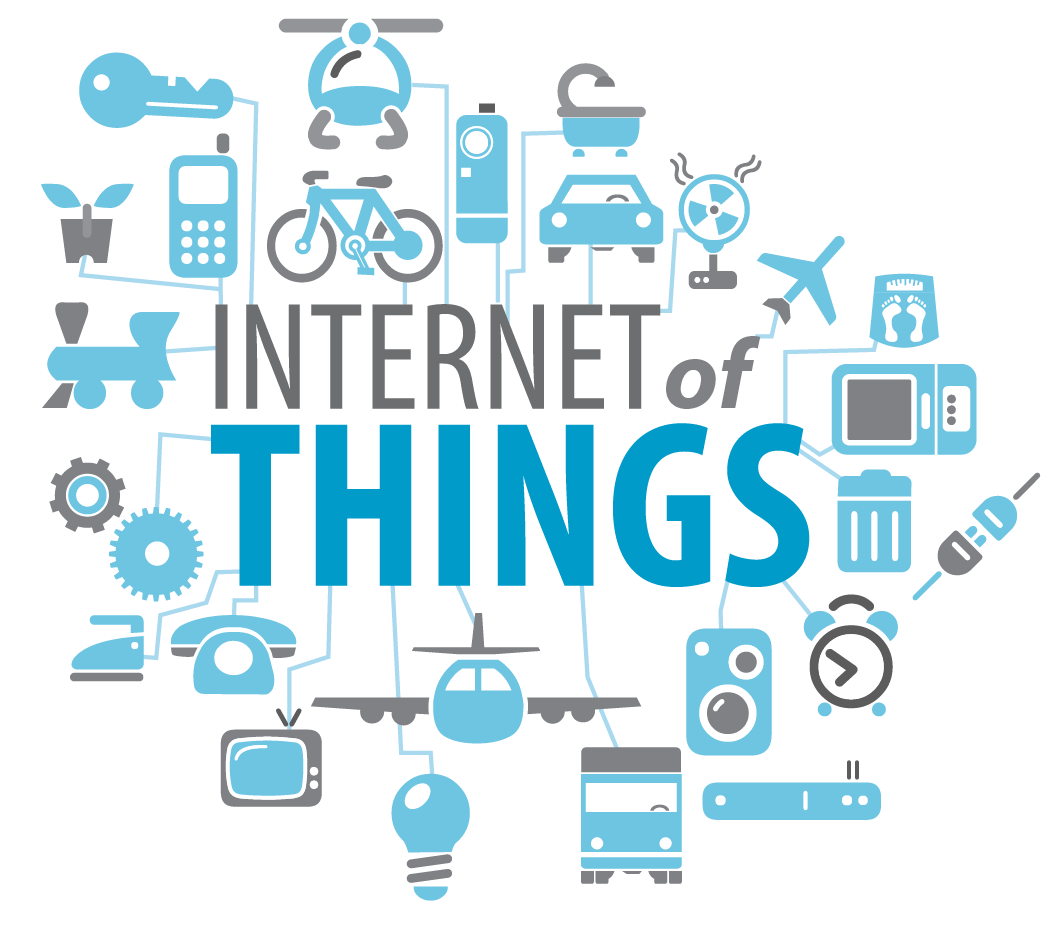
\includegraphics[width=8cm]{IoT}
    
\end{frame}




\begin{frame}{IoT Applications}

\begin{itemize}
    \item Smart home
\item Wearables
\item Smart City
\item Smart grids
\item Industrial Internet
\item Connected Car
\item Connected Health
\item Smart Retail
\item Smart Supply Chain
\item Smart Farming
\end{itemize}

\end{frame}

\begin{frame}{Top Free and Open Source IoT Projects}
    % https://www.linux.com/news/21-open-source-projects-iot
    \begin{itemize}
        \item AllSeen Alliance (Interoperability framework) 
        \item DeviceHive (Big Data analytics)
        \item DSA (Distributed Services Architecture)
        \item Eclipse IoT (Java-based rules-based routing engine)
        \item Kaa (scalable end-to-end IoT framework )
        \item Macchina.io (Web-enabled, modular and extensible JavaScript and C++ runtime)
        \item Open Connectivity Foundation (IoTivity)
        \item OpenIoT (Java-based connectivity framework)
        \item PlatformIO (Python-based suite for remote data access)
    \end{itemize}
    
\end{frame}

\begin{frame}{Rise of Linux: IoT-ready Hardwares}


\begin{multicols}{2}
    \begin{itemize}
        \item Yocto Project!!!
        \item Raspberry Pi
        \item Intel Edison
        \item Intel Joule
        \item BeagleBone Black
        \item Qualcomm DragonBoard 
        \item MinnowBoard MAX
        \item Orange Pi
    \end{itemize}
\end{multicols}    
      
        \centering
  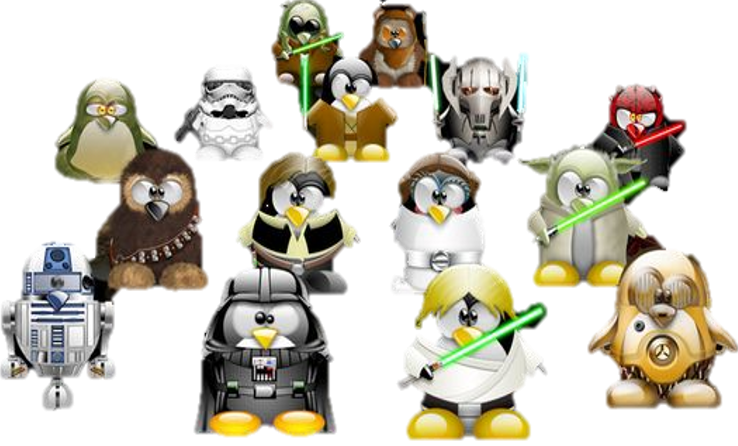
\includegraphics[width=7cm]{tux_star}
    
\end{frame}
    
    
    
\begin{frame}{IoT and Linux}

    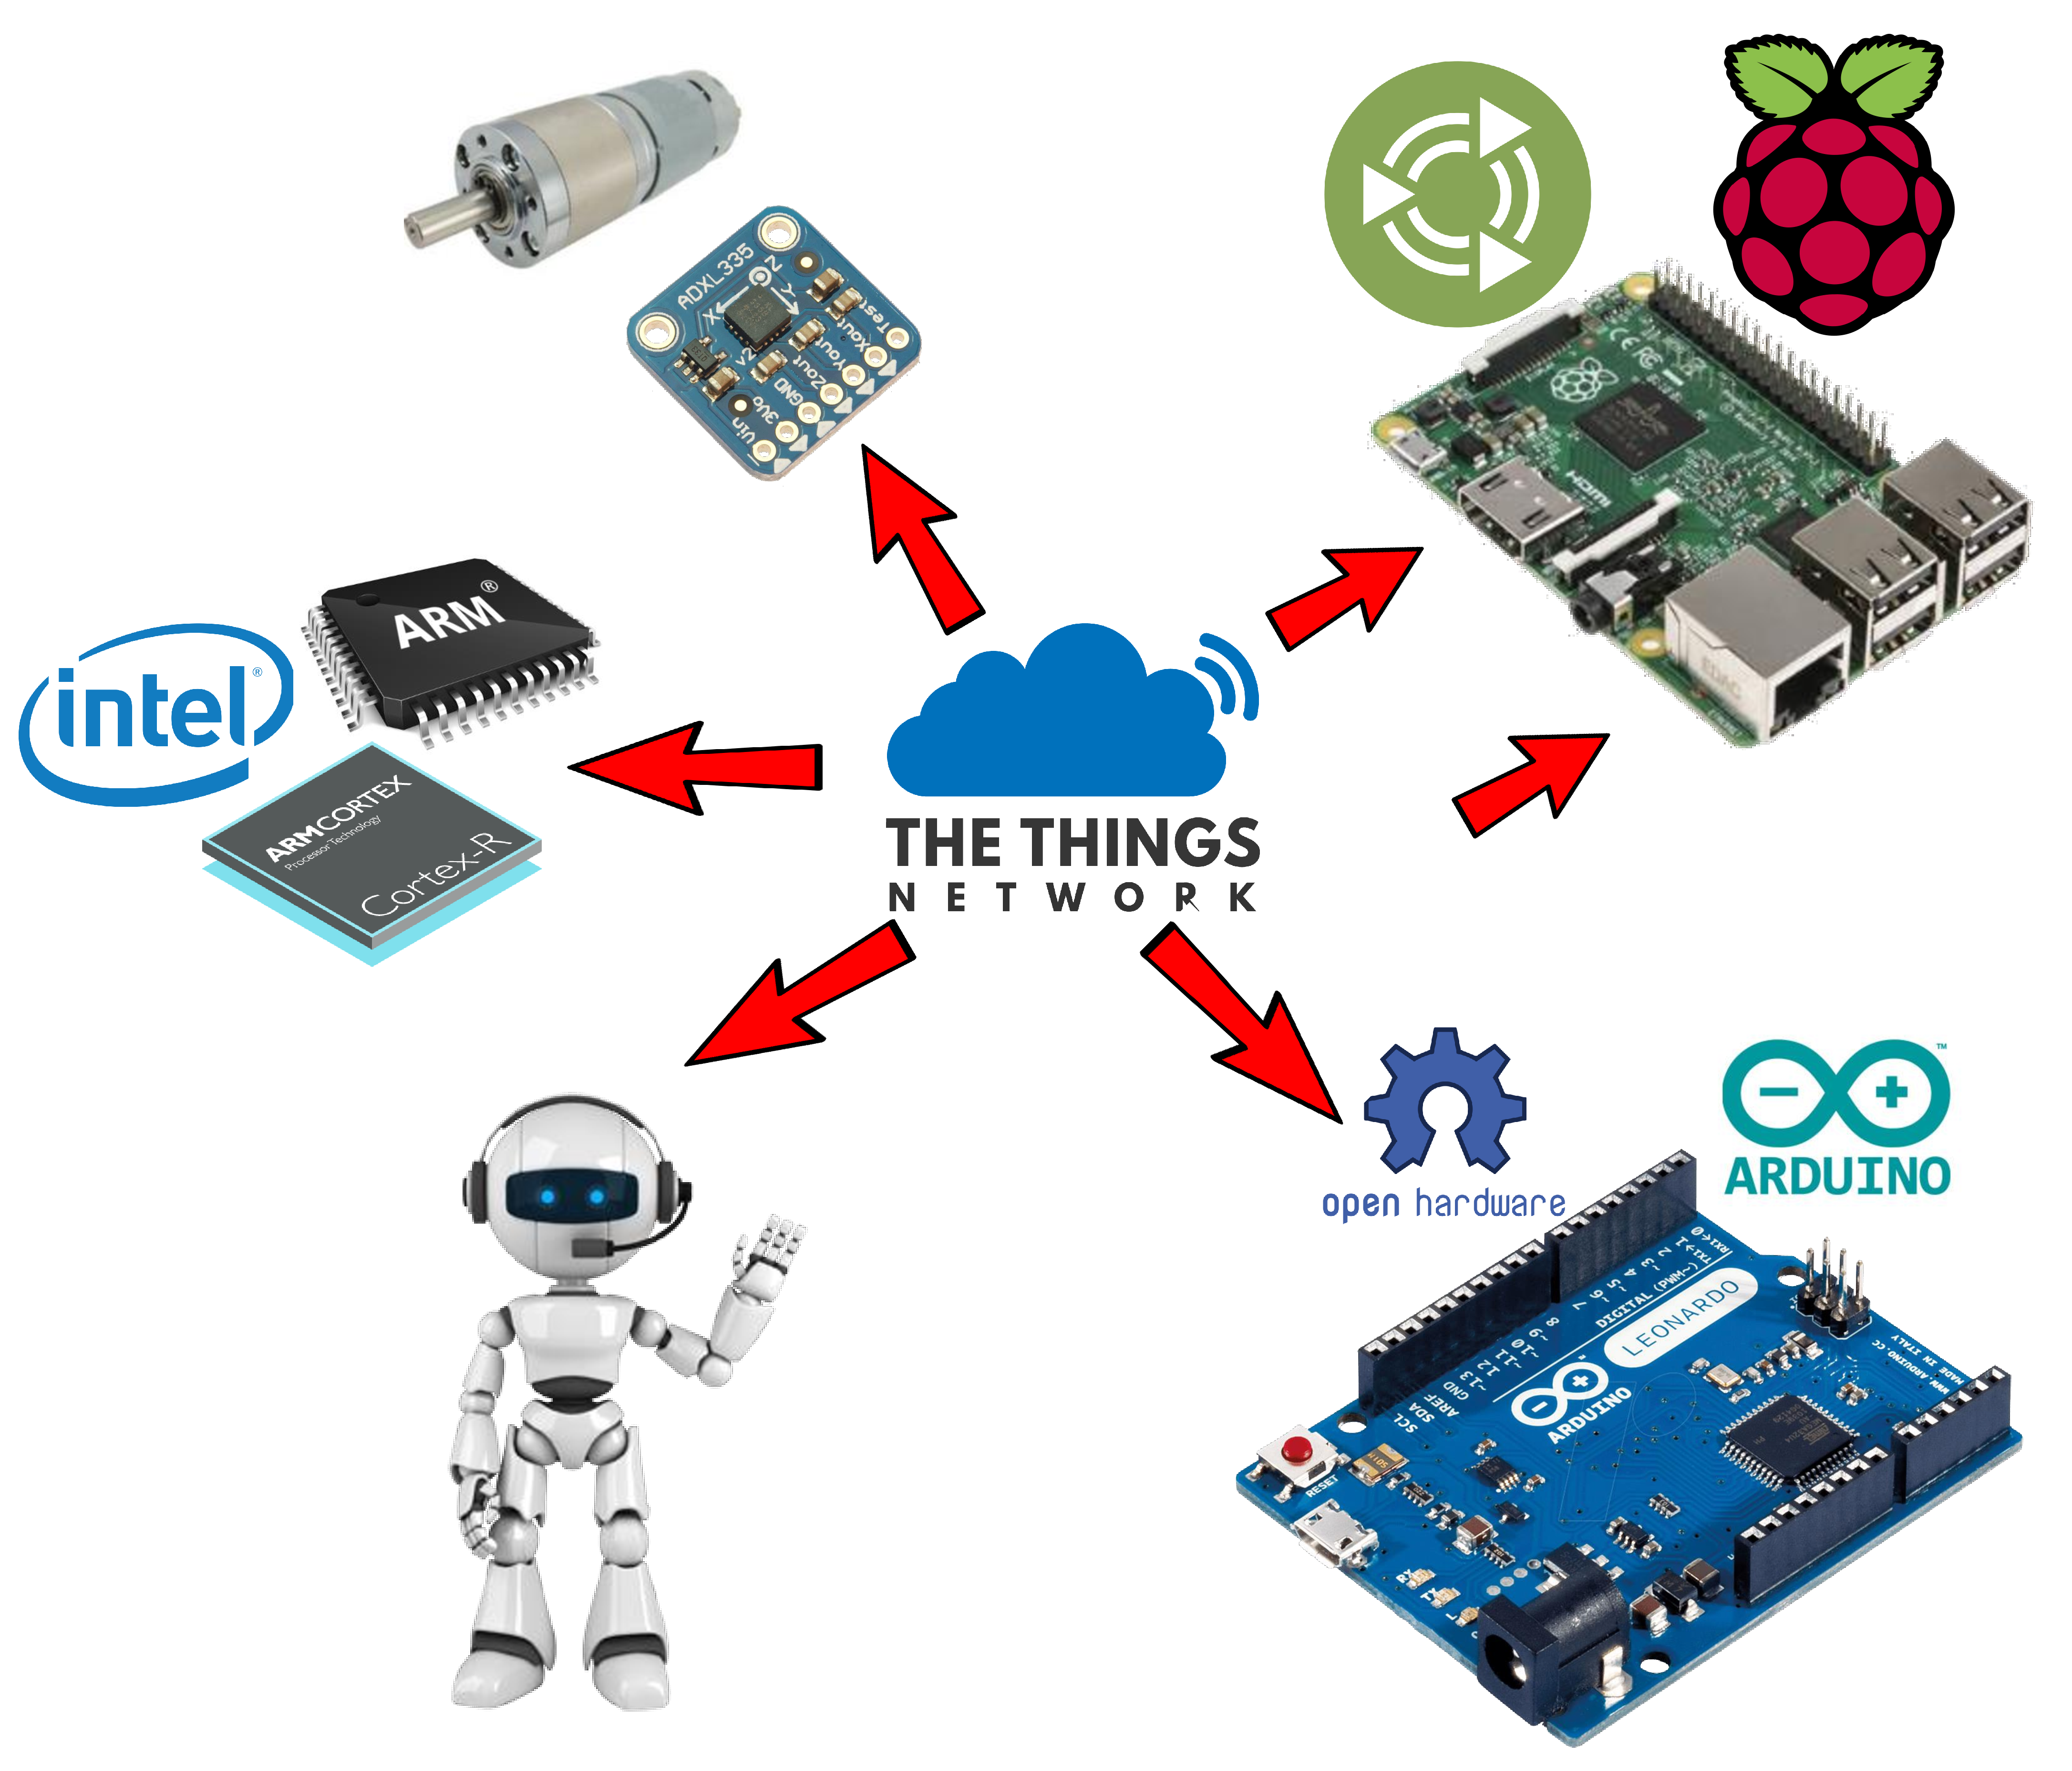
\includegraphics[width=8cm]{IoT_Linux}
    
\end{frame}


\begin{frame}{Raspberry Pi}

\begin{multicols}{2}

    \begin{itemize}
        \item
        \textbf{SoC}: Broadcom BCM2837
        \item
\textbf{CPU}: 4× ARM Cortex-A53, 1.2GHz
\item
\textbf{GPU}: Broadcom VideoCore IV
\item
\textbf{RAM}: 1GB LPDDR2 (900 MHz)
\item
\textbf{Networking}: Ethernet, 2.4GHz 802.11n wireless
\item
\textbf{Bluetooth}: Bluetooth 4.1 Low Energy
\item
\textbf{Storage}: microSD
\item
\textbf{GPIO}: 40-pin header
%\item
%\textbf{Ports}: HDMI, 3.5mm analogue audio-video jack, 4× USB 2.0, Ethernet, Camera Serial Interface (CSI), Display Serial Interface (DSI)
    \end{itemize}
    
    \end{multicols}
    
    \centering
    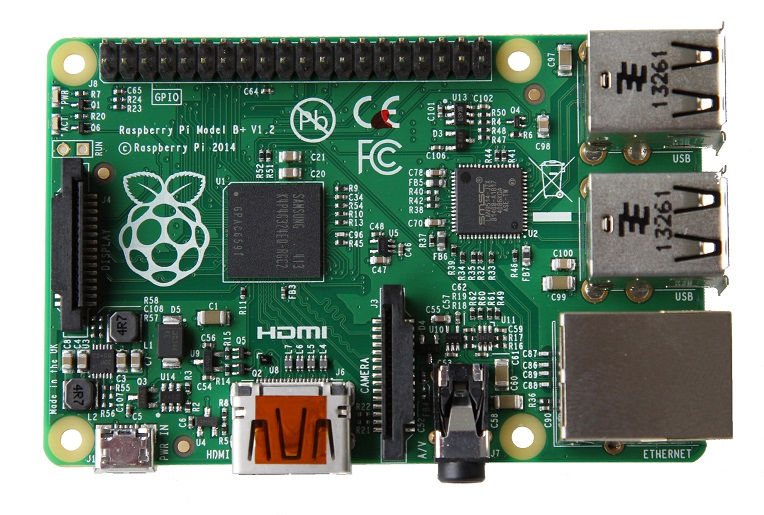
\includegraphics[width=5cm]{rpi}
    
\end{frame}



\begin{frame}{Intel Edison}

\begin{multicols}{2}

\footnotesize
\begin{itemize}
    \item
    \textbf{CPU}: Dual-core Intel Atom @500 MHz
    \item
\textbf{RAM}: 1 GB LPDDR3 
\item
\textbf{Storage}: 4 GB eMMC + micro SD card connector
\item
\textbf{Connectivity}:  Dual band Wi-Fi and Bluetooth 4.0
\item
\textbf{USB}: 1x micro USB connector
\item
\textbf{I/Os}:
\footnotesize
\begin{itemize}
    \item
2x UART  
\item
2x I2C 
\item
1x SPI with 2 chip selects
\item
1x I2S
\item
12x GPIO including 4 capable of PWM output
\end{itemize}
\end{itemize}

\end{multicols}

\centering
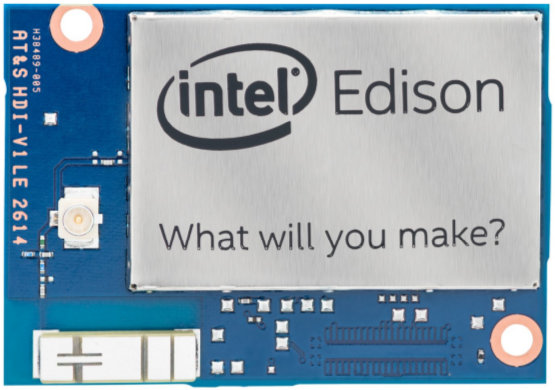
\includegraphics[width=3.5cm]{edison}

\end{frame}




\begin{frame}{Intel Joule}

\begin{itemize}
    \item
    \textbf{CPU}: Intel Atom T5700 64-bit quad-core @1.7GHz/2.4GHz
    \item
\textbf{RAM}: 4GB LPDDR4 RAM
\item
\textbf{GPU}: Intel HD Graphics with 4K video capture and display
\item
\textbf{Storage}: 16GB eMMC memory
\item
\textbf{Connectivity}: 802.11ac Wi-Fi with MIMO and Bluetooth 4.1
\end{itemize}

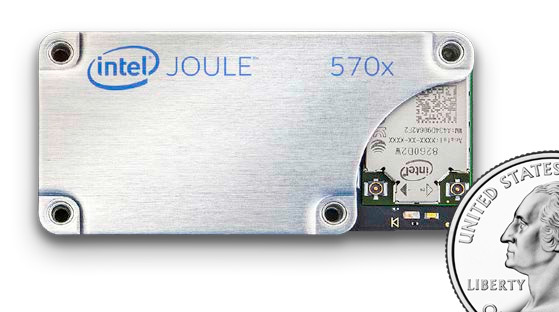
\includegraphics[width=5cm]{joule}


\end{frame}



\begin{frame}{Beyond the IoT: The Computation Thunderbolt }

These devices can be utilized in standalone computations:
\begin{itemize}
    \item Speech Recognition
    \item Machine Learning
    \item Image Processing
    \item Grid Computing
    \item Video Encoding/Decoding
\end{itemize}


\end{frame}